% =============================================================================
%  MAKALE METNİ / THE ARTICLE TEXT
% -----------------------------------------------------------------------------
%  Sadece metni yazın. Sayfa düzeni, süslemeler ve künye sizin işiniz değil.
%  Just write the text. Page layout, ornaments and front matter are handled
%  elsewhere -- see frontmatter.tex for page one.
%
%  Bölüm başlığı / a section heading:      \section{Bulgular}
%  Alt başlık / a subheading:              \subsection{...}
%  Alıntı / a block quotation:             \begin{quote} ... \end{quote}
%  Tablo, görsel / tables and figures:     see the examples below
%  Türkçe karakterler doğrudan yazılır -- ğ İ ı ş ç ö ü â
%  Yüzde işareti kaçışlıdır / percent must be escaped:  \%25,4
% =============================================================================

\section{Giriş}

Yapay zekâ, insan zekâsını gerektiren öğrenme, akıl yürütme, problem çözme,
örüntü tanıma ve karar verme gibi bilişsel süreçlerin bilgisayar sistemleri
aracılığıyla gerçekleştirilebilmesini sağlayan teknolojileri ifade etmektedir.
Makine öğrenmesi, derin öğrenme ve doğal dil işleme alanlarındaki
gelişmelerle birlikte yapay zekâ, son yıllarda birçok alanda hızla
yaygınlaşmış; sağlık sektörü de bu dönüşümden en fazla etkilenen alanlardan
biri olmuştur (Fahim vd., 2025; OECD, 2024).

Sağlık hizmetlerinde yapay zekâ; tanı, tedavi planlaması, hastalık öngörüsü,
ilaç geliştirme, kişiselleştirilmiş sağlık hizmetleri, hasta bakım yönetimi ve
klinik karar destek süreçlerinde kullanılma potansiyeli taşımaktadır. Ayrıca
halk sağlığı alanında salgınların erken tespiti, risk gruplarının belirlenmesi
ve sağlık kaynaklarının planlanması gibi konularda önemli fırsatlar sunmaktadır
(Alum \& Ugwu, 2025; DSÖ, 2025; Kaplan vd., 2024; Panteli vd., 2025). Bu
gelişmeler sağlık hizmetlerinden yararlanan toplumun yapay zekâya ilişkin
beklenti ve güven düzeyini önemli hale getirmektedir. Çünkü sağlık
hizmetlerinde yapay zekâ kullanımının sürdürülebilirliği ve başarısı, toplum
katılımı ve toplumun bu uygulamaları benimsemesi ile yakından ilişkilidir
(Osnat, 2025).

Son yıllarda yapay zekâ alanındaki ilerlemeler toplumun dikkatini çekmiş,
yapay zekâ uygulamalarının yaygınlaşmasıyla halkın konuya ilgisi artmıştır. Bu
ilgi, sağlık hizmetlerinde yapay zekâ uygulamalarının olası yararlarına ilişkin
beklentileri artırırken, bu uygulamaların risklerine yönelik kaygıları da
beraberinde getirmektedir. Daha hızlı hizmet, doğru tanı ve kolay erişim
beklentileri olumlu yönde etkilerken; mahremiyet, veri güvenliği, hatalı karar
verme ve etik sorunlar da kaygı yaratabilmektedir (Beets vd., 2023; Gundlack
vd., 2025). Bu bağlamda çalışmanın amacı, Balıkesir'de yaşayan yetişkinlerin
sağlık hizmetlerinde yapay zekâ kullanımına dair görüşlerini belirlemektir.

\section{Gereç-Yöntem}

Kesitsel tipteki bu çalışma için, Temmuz 2024'te Balıkesir Altıeylül ilçesi
merkez mahallelerinde yaşayan 18 yaş ve üzeri yetişkinlerden veri toplandı.
Araştırmanın evrenini Balıkesir ili Altıeylül ilçesinde yaşayan 18 yaş ve üzeri
107.052 yetişkin oluşturdu. Örneklem büyüklüğü Epi Info 7.2 programı
kullanılarak; \%95 güven aralığı, \%5 hata payı, \%50 sıklık, 1,5 desen etkisi
ve \%20 yedek ile 702 kişi olarak hesaplandı ve çok aşamalı küme örnekleme
yöntemiyle 715 kişiye ulaşıldı. Her mahalle, birer küme kabul edilip
ulaşılması gereken kişiler mahalle nüfusuna göre tabakalandırıldı. Basit
rastgele yöntem ile sokaklar belirlendi ve ilgili sokaklardan dört hane
seçildi. Her haneden bir kişi çalışmaya dahil edildi.

Anket görüşmeleri yüz yüze gerçekleştirildi. Anket için kâğıt baskı yerine
Google Forms platformu kullanıldı. Anket formu araştırmacılar tarafından
literatür taranarak oluşturuldu. Anket formu sosyodemografik özellikler; sağlık
durumu, alışkanlıklar, davranışlar ve teletıp deneyimi ile sağlık
hizmetlerinde yapay zekâ kullanımına ilişkin görüşlerden oluşmaktadır.
Toplanan veriler SPSS 26.0 programıyla çözümlendi. Tanımlayıcı veriler sayı ve
yüzde ile sunuldu. Kategorik değişkenlerin analizi için ki-kare testi, sürekli
değişkenlerin analizi için t testi kullanılmıştır. İstatistiksel anlamlılık
düzeyi p${<}$0,05 kabul edildi. Etik kurul onayı; Balıkesir Üniversitesi
Sağlık Bilimleri Girişimsel Olmayan Araştırmalar Etik Kurulundan alındı
(25/06/2024 tarih 2024/95 sayılı izin).

\section{Bulgular}

Katılımcıların yaş ortalaması 40,3 $\pm$ 15,3 olup \%52,9'u kadın, \%54'ü 50
yaş altında, \%50,8'i evli ve \%54,4'ü önlisans ve üzeri öğrenim düzeyine
sahipti. Katılımcıların \%53,6'sı herhangi bir işte çalışmakta, \%82,8'inin
hane geliri yoksulluk sınırının altındaydı. Katılımcıların sosyodemografik
özellikleri, sağlık durumları ve teletıp deneyimi ile ilgili bilgiler
Tablo~\ref{tab:sosyodemografik}'de sunulmuştur.

% -----------------------------------------------------------------------------
%  GENİŞ TABLO / a wide table
%  sosawide, sağdaki süsleme payını geri alır ve o sayfanın şeridini kaldırır.
%  sosawide reclaims the ornament reserve and drops that page's strip.
%  (İki kez derleyin / needs two compiles.)
% -----------------------------------------------------------------------------
\begin{table}[!ht]
\begin{sosawide}
\caption{Katılımcıların Sosyodemografik Özellikleri, Sağlık Durumu ve
         Teletıp Deneyimi}
\label{tab:sosyodemografik}
\centering
\begin{sosatabular}[\sosatablesmall]{@{}L{150pt}L{130pt}R{110pt}@{}}
\textbf{Değişkenler} &                    & \textbf{Sayı (\%)}    \\
\midrule
Yaş\textsuperscript{*} &                   & 40,3 $\pm$ 15,3       \\
\addlinespace[2pt]
\multirow{2}{*}{Yaş}   & 50 yaş altı       & 386 (\%54,0)          \\
                       & 50 yaş ve üzeri   & 329 (\%46,0)          \\
\addlinespace[2pt]
\multirow{2}{*}{Cinsiyet} & Erkek          & 337 (\%47,1)          \\
                       & Kadın             & 378 (\%52,9)          \\
\addlinespace[2pt]
\multirow{2}{*}{Medeni durum} & Bekar      & 352 (\%49,2)          \\
                       & Evli              & 363 (\%50,8)          \\
\addlinespace[2pt]
\multirow{2}{*}{Eğitim düzeyi} & Lise ve altı & 326 (\%45,6)       \\
                       & Önlisans ve üzeri & 389 (\%54,4)          \\
\addlinespace[2pt]
\multirow{2}{*}{Meslek} & Çalışmıyor       & 332 (\%46,4)          \\
                       & Çalışıyor         & 383 (\%53,6)          \\
\addlinespace[2pt]
\multirow{2}{*}{Hane geliri} & Yoksulluk sınırının altı & 592 (\%82,8) \\
                       & Yoksulluk sınırı ve üzeri & 123 (\%17,2) \\
\addlinespace[2pt]
\multirow{2}{*}{Çocuk varlığı} & Evet      & 393 (\%55,0)          \\
                       & Hayır             & 322 (\%45,0)          \\
\addlinespace[2pt]
\multirow{2}{*}{Kronik hastalık} & Evet    & 254 (\%35,5)          \\
                       & Hayır             & 461 (\%64,5)          \\
\addlinespace[2pt]
\multirow{2}{*}{İlaç kullanımı} & Evet     & 249 (\%34,8)          \\
                       & Hayır             & 466 (\%65,2)          \\
\addlinespace[2pt]
\multirow{2}{*}{Teletıp deneyimi varlığı} & Evet & 140 (\%19,6)    \\
                       & Hayır             & 575 (\%80,4)          \\
\end{sosatabular}

\vspace{2pt}
{\sosatablesmall \textsuperscript{*}Ortalama $\pm$ standart sapma}
\end{sosawide}
\end{table}

Katılımcıların \%64,5'i yapay zekânın tıpta faydalı olacağını düşünmekteydi.
\%44,8'i tıpta yapay zekânın doğru tanılar sunacağını düşünmekte ve \%57,3'ü
tıpta yapay zekâ kullanımında, kişisel verilerin güvenliği ile ilgili endişe
duymaktaydı. Katılımcıların sağlık hizmetlerinde yapay zekâ kullanımına
ilişkin bazı görüşleri Tablo~\ref{tab:gorusler}'de sunulmuştur.

% -----------------------------------------------------------------------------
%  NORMAL GENİŞLİKTE TABLO / a table that fits the ornament measure
% -----------------------------------------------------------------------------
\begin{table}[!ht]
\caption{Katılımcıların Sağlık Hizmetlerinde Yapay Zekâ Kullanımına İlişkin
         Bazı Görüşleri}
\label{tab:gorusler}
\begin{sosatabular}{@{}L{170pt}L{90pt}R{140pt}@{}}
\textbf{Değişkenler} & & \textbf{Sayı (\%)} \\
\midrule
\multirow{2}{170pt}{Sağlık hizmetlerinde yapay zekâ kullanımının faydalı
  olacağını düşünme}
                  & Evet     & 461 (\%64,5) \\
                  & Hayır    & 254 (\%35,5) \\
\addlinespace[4pt]
\multirow{3}{170pt}{Sağlık hizmetlerinde yapay zekânın doğru tanı sunacağını
  düşünme}
                  & Evet     & 320 (\%44,8) \\
                  & Kararsız & 248 (\%34,7) \\
                  & Hayır    & 147 (\%20,5) \\
\addlinespace[4pt]
\multirow{3}{170pt}{Sağlık hizmetlerinde yapay zekâ kullanımında kişisel
  verilerin güvenliği ile ilgili endişe duyma}
                  & Evet     & 410 (\%57,3) \\
                  & Kararsız & 196 (\%27,4) \\
                  & Hayır    & 109 (\%15,2) \\
\end{sosatabular}
\end{table}

Tablo~\ref{tab:gorusler}, sağlık hizmetlerinde yapay zekâ kullanımının faydalı
olacağını düşünen ve düşünmeyen bireylerin görüşlerini göstermektedir. Sağlık
hizmetlerinde yapay zekâ kullanımının faydalı olacağını düşünen bireylerin yaş
ortalaması (37,2 $\pm$ 14,4) düşünmeyenlere (45,7 $\pm$ 15,5) göre daha
düşüktü. Faydalı olacağını düşünme oranı 50 yaş altındakilerde \%73,8 iken,
50 yaş ve üzerindekilerde \%53,5'tir.

% -----------------------------------------------------------------------------
%  GÖRSEL / a figure
% -----------------------------------------------------------------------------
\begin{figure}[!ht]
  \centering
  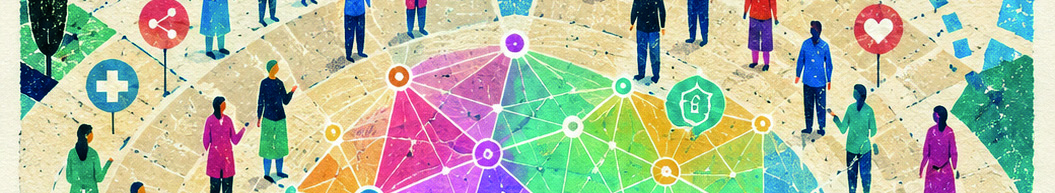
\includegraphics[width=0.62\textwidth]{assets/hero/hero-01}
  \caption{Yapay zekâya yönelik fayda algısının yaş gruplarına göre dağılımı}
  \label{fig:fayda}
\end{figure}

\section{Tartışma}

Bu çalışmada Balıkesir'de yaşayan yetişkinlerin yaklaşık üçte ikisinin sağlık
hizmetlerinde yapay zekâ kullanımını faydalı bulduğu saptanmıştır. Bu oran,
literatürdeki toplum tabanlı çalışmalarla benzerlik göstermektedir
(Aras vd., 2025; Busch vd., 2025). Bununla birlikte katılımcıların yarısından
fazlasının kişisel verilerin güvenliğine ilişkin endişe taşıması, mahremiyetin
kabul sürecindeki belirleyici rolüne işaret etmektedir
(Atalay \& Yücel, 2024; Esmaeilzadeh vd., 2021).

\begin{quote}
Alan yazında dijital sağlık uygulamalarının benimsenmesinde güvenin, algılanan
faydadan bağımsız biçimde belirleyici olduğu, özellikle veri paylaşımı söz
konusu olduğunda öne çıktığı bildirilmektedir.
\end{quote}

Çalışmanın Balıkesir ili Altıeylül ilçesi merkez mahallelerinde yürütülmüş
olması, bulguların diğer yerleşim yapılarına genellenebilirliğini
sınırlayabilir. Buna karşın çalışmanın toplum tabanlı olması ve yapay zekâya
yönelik fayda algısını sosyodemografik özelliklerle birlikte değerlendirmesi
önemli bir güçlü yönüdür.

\section{Sonuç ve Öneriler}

Sağlık hizmetlerinde yapay zekâya yönelik fayda algısı sosyodemografik
özellikler, sağlık durumu ve teletıp deneyimine göre değişmektedir. Toplumun
farklı gruplarına yönelik güven temelli, anlaşılır ve kanıta dayalı
bilgilendirme çalışmaları planlanmalıdır.
